%\documentclass[]{article}
%% 
%% Copyright 2007-2020 Elsevier Ltd
%% 
%% This file is part of the 'Elsarticle Bundle'.
%% ---------------------------------------------
%% 
%% It may be distributed under the conditions of the LaTeX Project Public
%% License, either version 1.2 of this license or (at your option) any
%% later version.  The latest version of this license is in
%%    http://www.latex-project.org/lppl.txt
%% and version 1.2 or later is part of all distributions of LaTeX
%% version 1999/12/01 or later.
%% 
%% The list of all files belonging to the 'Elsarticle Bundle' is
%% given in the file `manifest.txt'.
%% 
%% Template article for Elsevier's document class `elsarticle'
%% with harvard style bibliographic references

\documentclass[final,5p,times, twocolumn, sort&compress, sc]{elsarticle}

%% Use the options 1p,twocolumn; 3p; 3p,twocolumn; 5p; or 5p,twocolumn
%% for a journal layout:
%% \documentclass[final,1p,times]{elsarticle}
%% \documentclass[final,1p,times,twocolumn]{elsarticle}
%% \documentclass[final,3p,times]{elsarticle}
%% \documentclass[final,3p,times,twocolumn]{elsarticle}
%% \documentclass[final,5p,times]{elsarticle}
%% \documentclass[final,5p,times,twocolumn]{elsarticle}

%% For including figures, graphicx.sty has been loaded in
%% elsarticle.cls. If you prefer to use the old commands
%% please give \usepackage{epsfig}

%% The amssymb package provides various useful mathematical symbols
\usepackage[utf8]{inputenc}
\usepackage{textcomp}

\usepackage{graphicx}
\usepackage{float}
\usepackage{academicons}
\usepackage{orcidlink}
\usepackage{times}
\usepackage{color}
\usepackage{xcolor}
\usepackage{natbib} 
\usepackage{enumerate}
\usepackage{caption}
%\usepackage[separator = {;}]{credits}
\usepackage{lscape}
\usepackage{subcaption}
\usepackage{wrapfig}
\usepackage{orcidlink}
\usepackage{amssymb}
\usepackage{amsthm}
\usepackage{enumitem}
\usepackage{hyperref}
\hypersetup{colorlinks=true,
	citecolor=cyan,
	pdfauthor=cyan,
	linkcolor=cyan}

%opening


\begin{document}

%\maketitle
\begin{frontmatter}
	\title{Enhancing Space Activities in Africa and Maintaining Sustainability}
	\author[1]{Eshet Tafes\,\orcidlink{0000-0002-2743-4437}}
	%\fnmark[1]
	\corref{cor1}
	%\cortext[cor1]{Corresponding author}
	\ead{eshettesfaye377@gmail.com}
	
	\author[2]{Gadisa Dinaol}
	%\fnmark[2]
	%\corref{cor2}

	\affiliation[1]{organization={Department of Space Engineering, Space Science and Geospatial Institute },%Department and Organization
	addressline={Gulelle}, 
	city={Addis Ababa},
	postcode={33679}, 
	country={Ethiopia}}
	\affiliation[2]{organization={Department of Aerospace Engineering, Korean Advanced Institute of Science and Technology, KAIST},%Department and Organization
	addressline={291}, 
	city={Daejoen},
	postcode={34141}, 
	country={Republic of Korea}}


	\fntext[fn1]{Associate Researcher, Space engineering}
	\fntext[fn2]{PhD Candidate, Aerospace System and Control Lab}


\begin{abstract}
The rapid rise of space activities across Africa demonstrates the continent's rising curiosity in utilizing space technology for socioeconomic development and national security. This study examines at the current state of Africa's space programs, focusing on their accomplishments, challenges, and prospective for sustainable development. In addition, policy frameworks, international cooperation, and local capability development were also investigated to determine how African countries use space technology to address pressing issues such as poverty, resource management, and infrastructure development. The study also emphasizes the significance of a coordinated continental approach, in line with the African Union's Agenda 2030 and 2063, to ensure the long-term sustainability and impact of space activities. It is crucial to note that, while great progress has been made, more work is needed to create capacity, improve cooperation, and promote innovation in the African space sector, ultimately contributing to the continent's strategic goals and global competitiveness.
\end{abstract}
\begin{keyword}
	African space program \sep Agenda 2063 \sep Deep space exploration \sep Space infrastructure \sep 
	
\end{keyword}
\end{frontmatter}
\section{Introduction}
	Space exploration was mostly limited to a few industrialized countries, making it difficult for many emerging countries to engage actively. Consequently, public in space science and technology research and development in Africa didn't receive adequate policy or academic attention for decades. Despite this, Africa has shown interest in space exploration since the mid-20 century. Ethiopia, for instance, launched its first 4-inch optical telescope in 1957 and established the Addis Ababa Geophysical Observatory, a solar observation facility administered by Addis Abeba University's (AAU), ushering in the country's space program \cite{gadisa2023odyssey}. The chronological order of the South African space program also emphasizes that the program has been present since 1959, which began with an amateur rocketry group known as the South African Rocket Research Group (SARRG) \cite{gottschalk2010south}. Furthermore, a number of African nations launched space programs as part of their independence campaigns with the aim becoming technologically autonomous and use space technology to benefit the nation as a whole.
	
	The number of satellite payloads launched into space has increased considerably in recent decades. The United Nations Office for Outer Space Affairs (UNOOSA) \cite{andy2023} reports an increase in the number of space objects launched by new companies. According to the report, the total launches in 2020 and 2021 will account for nearly 25\% of all launched objects since the first satellite in the world was launched, indicating a significant engagement with space technology and services. The number of launches has risen to around 25 years after the first launch in 1957, and the number of satellites launched for emerging countries is rapidly increasing. As a result, the number of new nations entering the space sector, particularly those from developing nations, continues to rise, and many African governments, particularly two decades ago, established space organizations to support space endeavors on the continent. This clearly indicates how the space organization is now expanding and is accessible to developing nations.
	
	% Public space organizations were established and supported with space policies and objectives, especially through the African Union's (AU) Agenda 2030 and 2063 strategic plans for the continent. It strives to develop a legislative framework that supports Africa's space agenda and guarantees the continent's responsible and peaceful use of space [4]
	
	However, upto date, space-faring nations like the US, Russia, and China dominate satellite launches and research, leading to undemocratization of space exploration \cite{andy2023}. This is due to the fact that, non-space-faring nations lack enough space infrastructure, making it difficult for the continent to provide these services independently.
\section{African space program}
Africa's future is envisioned as \textit{ ".... an integrated, wealthy, and peaceful Africa, driven by its own skilled manpower and representing a powerful force in the global arena." \cite{union2017african} }. It is critical to emphasize that Africa, when compared to the industrialized world, has significant growth potential that can be fulfilled by seriously considering the use of cutting-edge technologies. In particular, the utilization of space science, technology, and its applications offers enormous potential for daily activities and the socioeconomic growth of the region in general. Subsequently, many African countries have recently been working to advance their space programs, including the development of satellite technology for a variety of uses such as remote sensing and communication. 
Currently, around 21 countries have established their own space agency, and fifteen of them own at least one satellite \cite{union2017african}. Several countries, including South Africa, Egypt, Algeria, Nigeria, Ethiopia, Ghana, Tunisia, and Kenya, have already launched satellites into space, while others are working on establishing  their own space programs. Figure \ref{fig:no_sat} illustrates the number of satellites launched by some of the African countries. 

\begin{figure*}
	\centering
	\includegraphics[width=.8\linewidth]{figs/Number of sat}
	\caption{Number of satellites launched by African countries}
	\label{fig:no_sat}
\end{figure*}

However, historically, the majority of these African satellites were launched from the territory of other nations, such as the United States, France, Russia, China, and Japan, using their launcher rockets, which cost a lot of foreign currency for the launching service and other businesses, including the spacecraft's development cost, launching insurance, and operational costs. Such expenses are substantial, and most governments' space budgets are insufficient to disperse the space budget, owing to the sector's limited national budget allocation.

Despite the fact that there was a common problem, such as a lack of awareness about the benefits of space technology for sustainable development and insufficient investment in the region's space sector, most countries now recognize that space-based services are far more useful to regional development by providing rapid and precise data. 

\subsection{\textbf{National and regional security}}
Space science and technology have significant contributions to national security, particularly for developing nations where maintaining security and prosperity is critical. In the contemporary world, role space technology in social, political, and economic activities is indispensable. Subsequently, many nations, particularly those with developing economies, invest in this sector, and new entrants can often be successful by using their newcomer advantage \cite{ehlers2016air}. 

Satellite technology provides numerous benefits, including space-based data and other applications that play an important role in resource management \cite{metzger2016space}. The existence of a space program itself enhances a nation's economic standing. For example, in India \cite{nair2006space}, the aerospace sector's ability to address security concerns is integral to its strategy for sustained growth and national development.

Space research and technology facilitate numerous applications, such as space surveillance, which is now a strategic priority for many African nations. This capability supports both regional and independent national security. In the near future, Africa is expected to emerge as a significant player with the potential to influence global socioeconomic activities. However, economic progress cannot be assured without a robust, autonomous, and internationally capable security force, which also necessitates international collaboration. This interdependence fosters a "balancing of interests," replacing the traditional "balance of power" with more complex politics of "competition and cooperation \cite{bediaerospace} 

Today, space science and technology are pivotal in supporting national security, particularly through satellite-based monitoring and reconnaissance. For African nations, this can bolster peacekeeping operations and enhance regional security cooperation. Although ideological divides persist, the importance of cooperative organizations and collective security has grown. Despite limited prevalence in African countries, weak policies have hindered participation in cooperative mechanisms and collective security organizations, especially in space-based security. Nevertheless, some nations are advancing their space-based national security initiatives, and there are indicators of a strategic plan for future synergy and unity across the continent.

\subsection{\textbf{Achieving agenda 2030 and 2063}}
As a strategic plan, the African Outer Space Flagship aims to develop a globally competitive, well-coordinated, and integrated continental program that addresses Africa's social, economic, political, and environmental needs. The African Union recently established the African Space Agency (HQ Egypt in January 2023) to promote cooperation between African member countries space policy and promote space activities on the continent. Both commercial and public space organizations are supported by relevant space policies and strategies that are in line with the African Union's (AU) Agenda 2030 and 2063 strategic plans. These initiatives aim to develop a legislative framework that supports Africa's space agenda while also ensuring the continent's responsible and peaceful use of space in accordance with international rules and treaties.

According to the African Union report, Agenda 2030 includes the United Nations' Sustainable Development Goals (SDGs), established in September 2015, with 17 objectives and 169 targets addressing various sustainable development challenges, such as poverty, inequality, climate change, environmental degradation, peace, and justice. These goals are consistent with the African Union's Agenda 2063, which serves as a roadmap for African countries to achieve sustainable development and improve the well-being of their citizens \cite{kabachinski2010laptops}. Agenda 2063 aims to reshape the continent's socioeconomic landscape from 2013 to 2063 by focusing on key sectors such as economic diversification, industrialization, infrastructure development, education, healthcare, and regional integration. It envisions a prosperous and peaceful Africa, driven by its people and acting as a dynamic force on the global stage. It emphasizes Africa taking ownership of its development agenda, promoting intra-African trade and collaboration, utilizing its resources for the benefit of its people, and building resilient and sustainable economies.
%According to African Union report, Agenda 2030, the United Nations' Sustainable Development Goals (SDGs), which were established in September 2015 with 17 objectives with 169 targets that can address a wide variety of sustainable development challenges, including poverty, inequality, climate change, environmental degradation, peace, and justice. It is a consistent with the goals of the African Union's Agenda 2063 that acts as a road map for African countries to achieve sustainable development and increase the nations' well-being[12]. Whereas the African Union's Agenda 2063 aims to reshape the continent's socioeconomic landscape from 2013 to 2063. It seeks to accelerate Africa's growth and development by concentrating on critical sectors such as economic diversification, industrialization, infrastructure development, education, healthcare, and regional integration. It aims to build a wealthy and peaceful Africa, led by its people and representing a dynamic force on the world stage. It underlines the need of Africa taking responsibility of its own development agenda, encouraging intra-African trade and collaboration, utilizing its resources for the benefit of its people, and developing resilient and sustainable economies.

Space-based activities are also integral to this strategic plan. Integrating a regional space program and its outputs with the frameworks of Agenda 2030 and Agenda 2063 can help Africa accelerate its growth and development. Many challenges have been addressed through collaborative efforts, and regional space activities are becoming increasingly vibrant and dynamic, achieving strategic goals. As part of this collective success, the African Space Agency was established and is now working for the region, although it is still in its early stages, particularly in areas such as outer space exploration.
%Space based activities are also the concern for the strategic plan and incorporating a regional space program and its outputs for the frameworks of Agenda 2030 and Agenda 2063 can help Africa to accelerate its growth and development in the region. To this end so many challenges have been solved through a collaborative effort with the nation and also the regional space activities are being one of the vibrant and dynamical that was achieving the strategic goals. As a collective success in the region African space agency was also established and now working for the region even though it still at infant stage particularly in the areas like outer space exploration.
\subsection{\textbf{International collaboration on deep space exploration mission}}
It is critical to emphasize that engaging in the global aerospace community promotes international collaboration and diplomacy, since many countries can form partnerships with other countries, space agencies, and international organizations to share knowledge, resources, and expertise.  A Collaborative efforts and initiatives, such as cooperative research projects, technology transfer agreements, and capacity-building programs, foster mutual understanding, cooperation, and peaceful coexistence in the pursuit of common goals. However, as space exploration advances, it is critical for African nations to engage more in research that enhances understanding and utilization of deep space and the lunar exploration.
\begin{figure*}
	\centering
	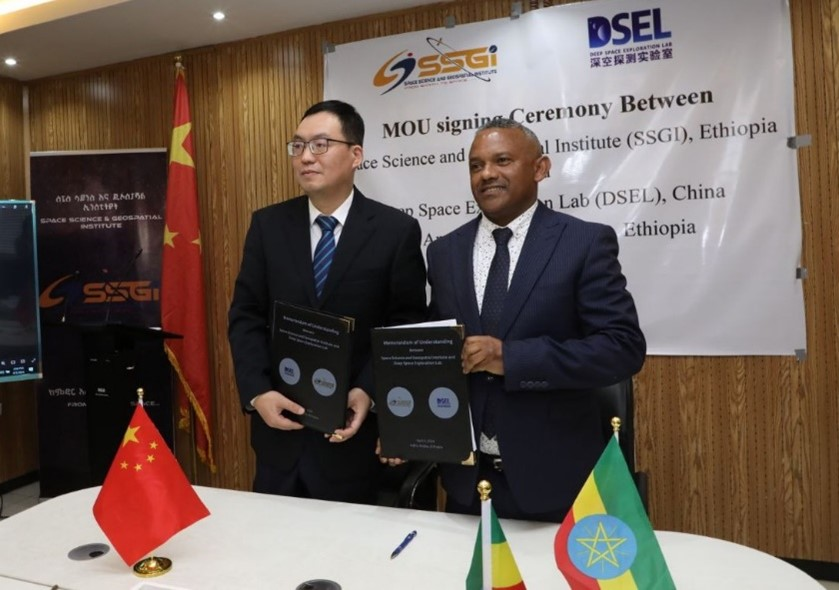
\includegraphics[width=.8\linewidth]{figs/lunar_mou}
	\caption{Agreement between Ethiopia and China in the realm of lunar exploration}
	\label{fig:luna}
\end{figure*}
A recent agreement between Ethiopia and China on lunar research (Figure \ref{fig:luna}) demonstrates that certain African countries have the desire to work with international space agencies and organizations, particularly in deep space exploration. According to the agreement, the collaboration's main goals are to: promote mutual growth and learning; facilitate the exchange of cutting-edge technologies and deep space exploration expertise; conduct joint research and development, including educational and training initiatives to develop a skilled workforce capable of leading deep space exploration initiatives; and establish a robust worldwide network through collaborative efforts, gatherings, and common goals to enhance our reputation in the space exploration community.

Furthermore, Egypt, South Africa, and Kenya are among the African countries that have signed a memorandum of understanding with the Chinese Deep Space Exploration Laboratory to work together on the International Lunar Research Station. 

%The ILRS includes twelve member countries, such as China, Russia, Venezuela, Pakistan, Azerbaijan, Belarus, South Africa, Egypt, and Thailand, along with numerous members from scientific institutions, universities, and businesses working to establish a permanent base on the moon by the mid-2030s.



%Participation in the global aerospace community facilitates international collaboration and diplomacy. Countries can forge partnerships with other nations, space agencies, and international organizations to share knowledge, resources, and expertise. Collaborative initiatives such as joint research projects, technology transfer agreements, and capacity building programs promote mutual understanding, cooperation, and peaceful coexistence in the pursuit of common goals. So far nations are more actively participating in the global space collaboration basically skilled manpower development. However, as space exploration advances, it is critical for African nations to be at the forefront of knowledge and do research that may lead to a better understanding and use of deep space and the moon. To that goal, numerous African governments are currently eager to collaborate with international space agencies and organizations throughout the world, notably in the field of deep space exploration. Ethiopia, for example, has already signed a memorandum of understanding with the Chinese Deep Space Exploration Laboratory to collaborate on the International Lunar Research Station (ILRS). Egypt, South Africa, and Kenya are among the African countries that have already signed the deal. 

%The ILRS has twelve member countries, including China, Russia, Venezuela, Pakistan, Azerbaijan, Belarus, South Africa, Egypt, and Thailand[13]. It also comprises numerous members from scientific institutions, colleges, and businesses working to establish a permanent base on the moon by mid-2030.

%According to the agreement the collaboration's main goals are to: Promote mutual growth and learning; facilitate the exchange of cutting-edge technologies and deep space exploration expertise; joint research and development, which includes working together on educational and training initiatives to develop a skilled workforce capable of leading the country's deep space exploration initiatives; establishing a robust worldwide network via collaborative efforts, gatherings, and common goals to improve our reputation in the space exploration community.
\subsection{\textbf{Space infrastructure and technological development}}
Several African countries are attempting to expand their space infrastructure, which includes satellite ground stations, launch facilities, teleports, astronomy, and assembly, integration, and testing infrastructure. 

Africa's space assets and infrastructure have grown dramatically as of the writing of this article, with the continent now home to 355 ground stations, 60 ground telescopes, 22 planetariums, and over 11 reowned observatories \cite{sa2023}. For example, in addition to launching their own satellite, Algeria recently established their own AIT facility \cite{momoh2008overview}, while other countries such as Ethiopia, South Africa, Nigeria, and Egypt are working hard to establish space infrastructure such as launch sites, space ports, and transportation systems. 
These will allow the region to establish and develop space technology while also increasing its own capabilities. In addition to regional capacity building, some countries began offering space science and technology education at various levels in order to fulfill their goals. For example, Ethiopia just began offering graduate degrees in space engineering, aeronautical engineering, and aerospace engineering. 

%On top of that new technological developments now is allowing for automated insights from space-based services for poverty rate monitoring, as well as the development of new Goals-relevant applications[15]. Recently the regional space program has the potential to propel the continent to the forefront of technological innovation. This technological advancement can have ripple effects across various sectors, driving economic growth and enhancing competitiveness on the global stage. The aerospace industry also has a capacity to incite economic growth and provide job opportunities in several domains. Moreover, the expansion of the aerospace industry may help downstream sectors like aviation, aerospace services, and tourism by creating jobs and boosting the economy.
\subsection{Investment of space program}
Africa is the second-largest continent after Asia, with 55 countries that comprise about 20\% of the world's population , a median age of 22 [21] and 1.4 billion people in 2023, which is next to Asia (4.7 billion). In 2013, African countries spent less than \$100 million \cite{union2017african} on space operations, accounting for less than 0.2\% of the global budget. 

Despite several setbacks in African space program, the region's space industry has maintained substantial expansion. According to Ref. \cite{sa2023}, the African space industry is expected to generate over USD 7 billion in annual revenues by 2019 and grow at a 7.3\% compound annual growth rate to exceed USD 10.24 billion by 2024 and USD 22.64 billion by 2026, with approximately 270 new space companies developing space technologies and offering space-enabled services to meet market demands in various sectors. 

Furthermore, Ref. \cite{sa2023} reveals that over USD 717 million spent on satellite projects to launch their own spacecraft, which was the best year in the history of the African space sector, and more than 100 additional satellites will be launched between now and 2025. Over USD 4 billion has been invested in satellite development and launch in Africa, allowing many new nations to join the race. Recently, Djibouti and Namibia are starting to establish their own domestic space programs, which can contribute to their efforts to compete in what could grow into a US\$10 billion market over the next two years. Additionally, Djibouti and China have signed an agreement to build a \$1 billion worthing spaceport in Djibouti, which will be jointly managed by China and Djibouti over a 30-year period.

%[24]. On the other hand, the Ethiopian government and Ethiopian Space Science and Geospatial Institute, then Ethiopian Space Science and Technology Institute are working on a national space port and launch site development in the near future. In this regard, the Ethiopian government, in collaboration with the national space institute, has been raising the national space budget in each fiscal year and investing funds from its national space budget for  On the other hand, in order to take advantage of their location on the continent, for instance, Ethiopia and Djibouti are on their way to establishing their space transportation and launch sites in their territories. For instance Djibouti and China have signed an agreement to build a \$1 billion worthing spaceport in Djibouti, which will be jointly managed by China and Djibouti over a 30-year period [24]. On the other hand, the Ethiopian government and Ethiopian Space Science and Geospatial Institute, then Ethiopian Space Science and Technology Institute are working on a national space port and launch site development in the near future. In this regard, the Ethiopian government, in collaboration with the national space institute, has been raising the national space budget in each fiscal year and investing funds from its national space budget for domestic space operations since 2017. According to a report from Ethiopian Space Science and Geospatial Institute, Ethiopia has been allocating an increasing amount of budget for the national space program. For instance, in 2017 and 2018, the national budget for the space program was about 1.1 million dollars, whereas in the 2022 and 2023 fiscal years, the national space budget was about 13 million dollars, which is a huge budget increment. On the other hand, Kenyan business executives have also investigated the viability of building a spaceport on the continent by investing a lot of budgets in the program. Zambia also plans to launch its first satellite in 2023, and Egypt is on track to build the Satellite City Industrialization and Assembly Center. These programs are all running with separate national space investment costs for each nation.

%Therefore, more or less, there are showcases that African countries are committed to working for their space programs by injecting more money for their national space programs. By 2022, there was an investment of USD 534.9 million in their domestic space programs [22]. When compared to the updated USD 523.3 million in 2021, this sum represented an increase of 2.24\%. This shows that the government's contributions grew from the revised USD 289.33 million in 2019 to USD 523.2 million. The growth of the satellite business on the continent is another indication that African governments want to rely on space-based services. In this regard, the establishment of an African space agency has been supported by the African Union (AU)[4-6], which governs almost the whole continent. According to AU law, a global space agency would allow AU countries to "harness space resources in a more coordinated and systematic manner" and "create an African space market".

%Above all, the African Space Agency (ASA) has prompted African countries to increase their space investment that can contribute to the continent's goals of smart, sustainable, and inclusive growth, which can be the best way to stimulate the growth of the continent in fields such as telecommunications, navigation, and Earth observation. Furthermore, to ensure independence and security issues in the nations through the resolution of significant social, political, and economic problems such as food insecurity, climate change across the continent.

\section{Regional achievements}
Africa and its member countries are working hard to establish a comprehensive and far-reaching African space program that has the potential to transform multiple dimensions, including technological advancement, scientific discovery, national security, economic development, education, and international cooperation. Furthermore, the African space program has reached a number of regional milestones, demonstrating the continent's growing capabilities and goals in space science and technology, which are crucial for addressing regional issues and contributing to global space endeavors. Some of the achievements include:
\subsection{ \textbf{Establishment of national space agency}}
	The establishment of space agencies in several African countries is a key step forward in the continent's path toward utilizing space science and technology for development. In particular, the African Union established the African Space Agency (AfSA) to coordinate and harmonize space operations among member countries, thereby encouraging regional collaboration and resource sharing. 
	
	Egyptian Space Agency, South Africa's National Space Agency (SANSA), Nigerian space research and development, Ethiopian Space and Geospatial Institute, Rwanda space agency, and Kenyan space agency, to name a few, are among the officially recognized and established by their respective countries and governments. They are instrumental in Earth observation, space weather monitoring, and satellite development, significantly contributing to the region's space capability.  These national agencies are not only advancing their respective countries space capabilities but also fostering international partnerships and collaborations, thereby enhancing Africa's overall presence in the global space sector.
\subsection{\textbf{Capacity building and education}}
	Space science and technology capacity building in various African countries are vital for developing a trained workforce and expanding the continent's space capabilities. The African Union's Space Science and Technology Strategy aims to expand competence through educational programs, scholarships, and research opportunities. For example, South Africa is host to the Pan-African University Institute for Space Sciences (PAUSS), which offers advanced training and research to students across the continent. 
	
	Countries such as Nigeria and Kenya are investing in university programs and forming relationships with international space agencies to improve their technical skills and knowledge capacity.  Furthermore, initiatives such as the African Resource Management Constellation (ARMC) provide hands-on training in satellite technology and Earth observation. These activities are critical for developing a strong space sector in Africa, allowing the continent to actively engage in global space endeavors while also utilizing space technology to local issues.
\subsection{\textbf{Growth of number of satellites}}
	The increasing number of satellites launched by various African countries demonstrates the continent's developing space capabilities and commitment to using space technology for development. Countries such as Nigeria, Egypt, South Africa, and Ethiopia have increased their satellite deployments dramatically during the last two decades. Furthermore, Egypt launched NILE 101 satellite in 1998, while South Africa launched SunSat-1 satellite in 1999, marking the first time in African satellite history. 
	
	Since 2016, African countries have launched around 21 satellites, and as of April 2023, the total number of satellites in the region reached around 58, launched by 15 African countries \cite{sa2023}. South Africa leads with 13 satellites, followed by Egypt with 12 satellites in Africa, with the remaining spacecraft owned by Algeria, Nigeria, Morocco, Mauritius, Angola, Ethiopia, Tunisia, Ghana, Sudan, Kenya, and Rwanda. Other African countries are also planning to launch their own satellites in the very near future, such as Tunisia, which will launch its CubeSat with a Japanese Kibo CUBE satellite grant program of JAXA in collaboration with UNOOSA that will be deployed from the ISS. The increasing number of satellites in Africa reflects an intentional desire to use space technology to address crucial socioeconomic issues and improve regional development.
	%\item Lauching  regional satellite constellation program 
\subsection{\textbf{Space application for development}}
	Space applications are accelerating development in many African countries by addressing major socioeconomic concerns and enhancing regional economy. Satellites give precise farming data, monitor crop health, and manage natural resources, all of which contribute to increased food security. Ethiopia, for example, uses its ETRSS-1 satellite \cite{gadisa2023odyssey} to anticipate the weather and organize agricultural operations. Countries such as Nigeria and South Africa use satellites for early warning systems and effective disaster response, which increases resilience to natural disasters. 
	
	Furthermore, 81 space application projects \cite{sa2023} are currently being conducted across the continent, with funding coming from African and foreign institutions. These initiatives use earth observation resources and satellite communications to solve a wide range of socioeconomic issues across the continent, including catastrophe monitoring, security, agriculture, land use and management, and forest management.
		
	These applications not only promote sustainable development, but also encourage regional collaboration, establishing Africa as a growing player in the global space community.
\subsection{\textbf{International collaborations}}
	International space collaboration has substantially enhanced the capacities in several African countries, promoting technological, research, and development developments. African countries such as Ethiopia, Egypt, and South Africa have formed collaborations with international space agencies such the Chinese National Space Administration (CNSA), NASA, and the European Space Agency (ESA).
	
	Ethiopia, for example, is collaborating with China's Deep Space Exploration Laboratory to work on the International Lunar Research Station (ILRS) (Figure \ref{fig:luna}). Similarly, Egypt and South Africa have various bilateral agreements that allow for technology transfer, joint missions, and capacity-building projects. 
	
	These collaborations not only improve African countries' technical knowledge and infrastructure, but also foster peaceful cooperation and mutual growth within the global space community, allowing Africa to play a more important role in global space exploration endeavors.
\subsection{\textbf{Policy and regulatory framework}}
	African countries are increasingly establishing space policies and regulatory frameworks to support their burgeoning space sectors. The African Union's African Space Policy and Strategy provides a cohesive framework that encourages coordinated space activities across the continent. Furthermore, countries like Nigeria, South Africa, and Egypt have developed national space policies to regulate and guide their space endeavors. These policies focus on ensuring compliance with international laws and treaties, promoting peaceful uses of space, and fostering sustainable development. 
	
	Additionally, about 19 African nations such as: Algeria, Benin, Burkina Faso, Egypt, Equatorial Guinea, Kenaya, Nigeria, Tunisia are some nations have ratified the outer space agreement as of January 1, 2020; the remaining 10 had signed but not yet finished the ratification process.  On the other hand, some African countries such as Ethiopia, Botswana, Burundi, Gambia, Rwanda, Cameroon, are already signed the agreement but still need ratification. Given that as a continent so far more than half of the countries which is about 53\% of African nations have ratified or signed the agreement \cite{at2023}.
	%The legislative document states about how to explore the outer space in the context of public international laws and was prepared on January 27, 1967, under UN auspices and became available for signing in the US, the UK, and the USSR which went into effect on October 10, 1967 [17].
	
	%The 1967 treaty was more focused on the how to govern the outer space activities by different nations basically during space exploration including the moon and other celestial bodies. Ut it was not the first treaty during that time, there was also a 1963 agreement which was focused on the not to use to test a nuclear weapon.  Since then, different treaties have been developed and signed by different nations. In 1968 the United Nations committee for the peaceful use of the outer space treaty was amended which is basically regarding the rescue and return of astronauts and space objects. There are also different international outer space treaties have been signed. For instance, the 1972 which was about the international liability for damage, the 1979 regarding activities on the moon, 1982 and 1986 respectively states activities related to satellite communications and direct broadcasting and remote sensing and earth observation activities[16].  However, the first and most important piece of space legislation is the Outer Space Treaty which is the 1967 treaty, whose larger goals of advancing the peaceful and civil use of space continue to guide global space activities. However still Aerospace capabilities must be considered in a more recent and comprehensive context [17].
	
	%Different countries have their own national regulatory frameworks to control the conduct of space-related activities in addition to implementing international space law instruments. Therefore, even if they lack the technological ability to fully engage in space-related activities, like space-faring nations, most space-emerging nations in Africa have up to now found it important to adopt or ratify own space laws[18]. About 19 African nations such as: Algeria, Benin, Burkina Faso, Egypt, Equatorial Guinea, Kenaya, Nigeria, Tunisia are some nations have ratified the outer space agreement as of January 1, 2020; the remaining 10 had signed but not yet finished the ratification process.  On the other hand, some African countries such as Ethiopia, Botswana, Burundi, Gambia, Rwanda, Cameroon, are already signed the agreement but still need ratification. Given that as a continent so far more than half of the countries which is about 53\% of African nations have ratified or signed the agreement [18].
	
	%To this end most African countries already have their own national space policies that support their national space programs which aligned with the international agreements. For instant Ethiopia amended its space policy in 2020, as did Nigeria and South Africa, which had their own space policies prior to joining other African nations. Tunisia and Senegal are among the countries that are working on policies and strategies. Even some nations are still drafted their polices in considering the private sector as well to support the private enterprises. This is a showcases that the role of governmental agencies in the development of space technology, as well as commercial low-cost space operators that will allow for new forms of public-private collaborations[15]. The strategy also has a strong support Africa’s space industry goal towards supporting Agenda 2063 of the AU science and technology plan for Africa.
 	By establishing clear regulatory frameworks, African countries aim to enhance their space capabilities, encourage international collaboration, and ensure the responsible use of space technology for socio-economic growth.

%It was African strategic plan that by using the potential of space technology and innovation, African countries can open new prospects for growth and wealth, which can determine the continent's future and role in the global community.The nations of the continent are working both independently and in common via the African Union (AU), which has expressly called for Agenda 2063. The objectives outlined in Agenda 2063 of the African Union (AU) make a substantial contribution to the execution of the Science, Technology, and Innovation Strategy for Africa (STISA) [4], [15]. This plan's primary focus is on capitalizing on new possibilities made available by the geographical advantages held by the nations that make up the continent that makes a major contribution to the execution of the STISA. To this end the nations are in a remarkable progress to achieve the strategic goal which so far so many activities have been done basically through African union which is an indication for how the nation is committed for the areas.  
%\subsection{Space policies, laws and international treaties}
%Space law is the existing space legal system in the world that declares about activities in the outer space[16]. According to [17] till march 2024 about 115 nations are joined the international outer space treaties, of these countries still from the developing nations which is a showcases for the less participating of the developing nations. The legislative document states about how to explore the outer space in the context of public international laws and was prepared on January 27, 1967, under UN auspices and became available for signing in the US, the UK, and the USSR which went into effect on October 10, 1967 [17].

%The 1967 treaty was more focused on the how to govern the outer space activities by different nations basically during space exploration including the moon and other celestial bodies. Ut it was not the first treaty during that time, there was also a 1963 agreement which was focused on the not to use to test a nuclear weapon.  Since then, different treaties have been developed and signed by different nations. In 1968 the United Nations committee for the peaceful use of the outer space treaty was amended which is basically regarding the rescue and return of astronauts and space objects. There are also different international outer space treaties have been signed. For instance, the 1972 which was about the international liability for damage, the 1979 regarding activities on the moon, 1982 and 1986 respectively states activities related to satellite communications and direct broadcasting and remote sensing and earth observation activities[16].  However, the first and most important piece of space legislation is the Outer Space Treaty which is the 1967 treaty, whose larger goals of advancing the peaceful and civil use of space continue to guide global space activities. However still Aerospace capabilities must be considered in a more recent and comprehensive context [17].

%Different countries have their own national regulatory frameworks to control the conduct of space-related activities in addition to implementing international space law instruments. Therefore, even if they lack the technological ability to fully engage in space-related activities, like space-faring nations, most space-emerging nations in Africa have up to now found it important to adopt or ratify own space laws[18]. About 19 African nations such as: Algeria, Benin, Burkina Faso, Egypt, Equatorial Guinea, Kenaya, Nigeria, Tunisia are some nations have ratified the outer space agreement as of January 1, 2020; the remaining 10 had signed but not yet finished the ratification process.  On the other hand, some African countries such as Ethiopia, Botswana, Burundi, Gambia, Rwanda, Cameroon, are already signed the agreement but still need ratification. Given that as a continent so far more than half of the countries which is about 53\% of African nations have ratified or signed the agreement [18].

%To this end most African countries already have their own national space policies that support their national space programs which aligned with the international agreements. For instant Ethiopia amended its space policy in 2020, as did Nigeria and South Africa, which had their own space policies prior to joining other African nations. Tunisia and Senegal are among the countries that are working on policies and strategies. Even some nations are still drafted their polices in considering the private sector as well to support the private enterprises. This is a showcases that the role of governmental agencies in the development of space technology, as well as commercial low-cost space operators that will allow for new forms of public-private collaborations[15]. The strategy also has a strong support Africa’s space industry goal towards supporting Agenda 2063 of the AU science and technology plan for Africa.

%\subsection{Growth of number of satellite} 
%Due to Africa's long-standing interest in space research, the number of satellites launched by its countries is rapidly rising. After the launch of the first African satellites, NILE 101 by Egypt in 1998 and SunSat-1 by South Africa in 1999, the space industry in Africa became more focused on issue. However, due to the large investment in the design, development, and launch of a satellite, only a limited number of nations on the continent are participating in the space race. Despite the significant expense, since 2016, African countries have launched more than 21 satellites, which indicates an increment in the total number of satellites launched by Africans. Until April 2023, the total number of satellites [19] in the region reached about 58, which were launched by 15 African countries [20], including the CubeSats, which were launched in November 2022 by the two African countries of Uganda and Zimbabwe. Both Zimbabwe and Uganda launched their respective first satellites into orbit, which are part of the Joint Global Multi-Nation Bird Satellite Project of JAXA. According to the report, nine of those satellites were launched by commercial entities[19].

%As of the data, each of the 15 countries in the region contributes a particular percentage to the total number of regional satellites in Africa determined by the number of satellites that each country currently has in orbit.
%South Africa leads with 13 satellites, while Egypt takes second place with 12 satellites in Africa based on satellite number[20] whereas countries like Algeria, Nigeria, Morocco, Mauritius, Angola, Ethiopia, Tunisia, Ghana, Sudan, Kenya, and Rwanda own the remaining satellites. Other African countries are also planned to launch their own satellites in the very near future, such as Tunisia, which will launch its CubeSat with a Japanese Kibo CUBE satellite grant program of JAXA in collaboration with UNOOSA that will be deployed from the ISS which will be its second satellite for Tunisia. 


%\section{Challenges and opportunities of African space program}
%\subsection{Challenges}
%Even though the African space program is showing advancement, it encountered different challenges where these challenges are having a substantial impact on the development of the continental space program. Particularly on the capacity of newly entered countries and also for previously entered countries in the region to advance their existing space activities as well. The most commonly mentioned issues include a lack of indigenous skilled man powers, insufficient funding, political instability, lack of proper space infrastructure. And off course still lack of awareness is another obstacle that must be overcome.
%
%In the Africa the majority of the satellites launched by the 15 distinct nations were earth observation; EO satellites, where nearly all of which were launched from outside of the continent with huge amount of launching service cost. At the same time Africa still has the largest number of countries that have not signed or ratified space treaties and international space laws. National space policies and domestic legislation regulating space-related activities are similarly a handful in African nations[18].
%
%These challenges have been acknowledged; number of different policy frameworks have been developed as a response. The nations of the continent are working both independently and in common with one another via the African Union (AU), which has expressly called for Agenda 2063, which strongly supports the continent space program. The objectives outlined in Agenda 2063 of the African Union (AU) make a substantial contribution to the execution of the Science, Technology, and Innovation Strategy for Africa (STISA)[4] basically on capitalizing a new possibilities made available by the geographical advantages held by the nations. Implementation of the strategy is allowing Africa to emerge as the potential player in the space sector around the globe. As a consequence of this, African Union's Agenda 2063 make a major contribution to the execution of the STISA.
%\subsection{Opportunities}
%The goal for Africa's future is to be "an integrated, wealthy, and peaceful Africa, driven by its own local skilled man powers and representing a powerful force in the global arena. Africa, in comparison to the industrialized world, has a significant development potential, and this potential capitalized to construct a prosperous future for every nation in the region. In this sense, African nations awarded of the numerous benefits of space science and technology.  Numerous policy frameworks have been developed in response to these issues, which have long been acknowledged. Through the African Union (AU), which has a specific AU agenda for 2063, countries on the continent are working both independently and together to solve these concerns. Nevertheless, beyond just considering the advantages, courageous steps taken to cultivate the indigenous capacities and skills essential for self-sufficiency and the capacity building for the sustainable prosperity. To achieve and progress in the space industry, the region of Africa has also put a strong focus on participating on the outer space related issues as contributor and also has to develop state of the art national and reginal policies and strategies related to the space sector. 
%So far it is well known that most countries are working focused on building indigenous capacities such as: skilled manpower development, infrastructures that will help with the development of human, scientific, technological, organizational, and institutional resources and capabilities; creating facilities, programs, and the ability to evaluate and answer important questions about policy choices and ways of putting them into action. However, for the continued growth and improvement of the existing space activities inside the region, each country still needs to put more effort into concentrating on the fundamentals. In this respect, based on the experiences of the space fairing countries, to establish a powerful continental space program in the long term, each country needs to work more than they did so far, essentially concentrating on but not limited to:
%\begin{itemize}
%	\item Skilled Manpower Development: As the basis for an independent space program, the production of indigenous knowledge, with a primary emphasis on passing that information on to subsequent generations, should be a top strategic goal. The potential of the African space program is greatly helped by the presence of indigenous talent. In this respect, several African countries, such as Ethiopia, South Africa, and Nigeria, already had their own academic programs, albeit the emphasis of these programs was mostly on scientific research. It has been a year since countries like Ethiopia started providing master's and doctoral degree programs in aerospace and aeronautical engineering for their respective citizens.
%	\item Space Policy: Most African countries already have their own national space policies that support their national space programs. Ethiopia amended its space policy in 2020, as did Nigeria and South Africa, which had their own space policies prior to other African nations. Tunisia and Senegal are among the countries that are working on policies and strategies. However, still many nations are remaining. 
%	\item Launch Site and Launch Vehicle Development: In the long term, some countries are planing to participate in the aerospace industry, and the majority of the countries are launching their own spacecraft into orbit. As a consequence, the conventional method that African countries were employing to launch their spacecraft might be changed to the finest method, including considering the long-term plan of the continent. To accomplish the intended aim, the continent needs its own launch pad, spaceport, and launch vehicle; otherwise, it will continue to be reliant on other nations, which has a significant impact on their participation in space operations. A launching site is now necessary for Africa as a continent, based on the recent major development in its satellite launching program. African nations need to have a launching facility that is best for delivering to orbit in a short period of time, reasonably priced, and appropriate for regular launch operations inside the continent's borders. The good news is that some of the nation’s provide excellent and suitable venues for constructing the center.
%\end{itemize}
\section{Conclusion}
Africa is making great strides toward improving its space activities and ensuring sustainability, primarily through measures spearheaded by the African Union. However, establishing a unified African space program remains an important step which has been already achieved. Space services are currently not widely used across the continent, with only a few countries actively involved. To achieve long-term sustainability, all African countries must support and participate in space initiatives, including changing regional laws and regulations. Developing regional space capabilities has been difficult, but it is critical to furthering Africa's economic, political, environmental, and societal objectives. Key measures include allocating adequate budgets, developing indigenous capacity, encouraging international cooperation, and promoting global collaborations. Furthermore, having a flexible curriculum and providing ongoing education and training are critical for developing a skilled workforce.  These initiatives will help to ensure the sustainability and dependability of space activities, as well as the establishment of competitive public and commercial space businesses in Africa.

\bibliographystyle{unsrt} 
\bibliography{sample}

\end{document}
